% Options for packages loaded elsewhere
\PassOptionsToPackage{unicode}{hyperref}
\PassOptionsToPackage{hyphens}{url}
\PassOptionsToPackage{dvipsnames,svgnames,x11names}{xcolor}
%
\documentclass[
  letterpaper,
  DIV=11,
  numbers=noendperiod]{scrartcl}

\usepackage{amsmath,amssymb}
\usepackage{iftex}
\ifPDFTeX
  \usepackage[T1]{fontenc}
  \usepackage[utf8]{inputenc}
  \usepackage{textcomp} % provide euro and other symbols
\else % if luatex or xetex
  \usepackage{unicode-math}
  \defaultfontfeatures{Scale=MatchLowercase}
  \defaultfontfeatures[\rmfamily]{Ligatures=TeX,Scale=1}
\fi
\usepackage{lmodern}
\ifPDFTeX\else  
    % xetex/luatex font selection
\fi
% Use upquote if available, for straight quotes in verbatim environments
\IfFileExists{upquote.sty}{\usepackage{upquote}}{}
\IfFileExists{microtype.sty}{% use microtype if available
  \usepackage[]{microtype}
  \UseMicrotypeSet[protrusion]{basicmath} % disable protrusion for tt fonts
}{}
\makeatletter
\@ifundefined{KOMAClassName}{% if non-KOMA class
  \IfFileExists{parskip.sty}{%
    \usepackage{parskip}
  }{% else
    \setlength{\parindent}{0pt}
    \setlength{\parskip}{6pt plus 2pt minus 1pt}}
}{% if KOMA class
  \KOMAoptions{parskip=half}}
\makeatother
\usepackage{xcolor}
\setlength{\emergencystretch}{3em} % prevent overfull lines
\setcounter{secnumdepth}{-\maxdimen} % remove section numbering
% Make \paragraph and \subparagraph free-standing
\makeatletter
\ifx\paragraph\undefined\else
  \let\oldparagraph\paragraph
  \renewcommand{\paragraph}{
    \@ifstar
      \xxxParagraphStar
      \xxxParagraphNoStar
  }
  \newcommand{\xxxParagraphStar}[1]{\oldparagraph*{#1}\mbox{}}
  \newcommand{\xxxParagraphNoStar}[1]{\oldparagraph{#1}\mbox{}}
\fi
\ifx\subparagraph\undefined\else
  \let\oldsubparagraph\subparagraph
  \renewcommand{\subparagraph}{
    \@ifstar
      \xxxSubParagraphStar
      \xxxSubParagraphNoStar
  }
  \newcommand{\xxxSubParagraphStar}[1]{\oldsubparagraph*{#1}\mbox{}}
  \newcommand{\xxxSubParagraphNoStar}[1]{\oldsubparagraph{#1}\mbox{}}
\fi
\makeatother

\usepackage{color}
\usepackage{fancyvrb}
\newcommand{\VerbBar}{|}
\newcommand{\VERB}{\Verb[commandchars=\\\{\}]}
\DefineVerbatimEnvironment{Highlighting}{Verbatim}{commandchars=\\\{\}}
% Add ',fontsize=\small' for more characters per line
\usepackage{framed}
\definecolor{shadecolor}{RGB}{241,243,245}
\newenvironment{Shaded}{\begin{snugshade}}{\end{snugshade}}
\newcommand{\AlertTok}[1]{\textcolor[rgb]{0.68,0.00,0.00}{#1}}
\newcommand{\AnnotationTok}[1]{\textcolor[rgb]{0.37,0.37,0.37}{#1}}
\newcommand{\AttributeTok}[1]{\textcolor[rgb]{0.40,0.45,0.13}{#1}}
\newcommand{\BaseNTok}[1]{\textcolor[rgb]{0.68,0.00,0.00}{#1}}
\newcommand{\BuiltInTok}[1]{\textcolor[rgb]{0.00,0.23,0.31}{#1}}
\newcommand{\CharTok}[1]{\textcolor[rgb]{0.13,0.47,0.30}{#1}}
\newcommand{\CommentTok}[1]{\textcolor[rgb]{0.37,0.37,0.37}{#1}}
\newcommand{\CommentVarTok}[1]{\textcolor[rgb]{0.37,0.37,0.37}{\textit{#1}}}
\newcommand{\ConstantTok}[1]{\textcolor[rgb]{0.56,0.35,0.01}{#1}}
\newcommand{\ControlFlowTok}[1]{\textcolor[rgb]{0.00,0.23,0.31}{\textbf{#1}}}
\newcommand{\DataTypeTok}[1]{\textcolor[rgb]{0.68,0.00,0.00}{#1}}
\newcommand{\DecValTok}[1]{\textcolor[rgb]{0.68,0.00,0.00}{#1}}
\newcommand{\DocumentationTok}[1]{\textcolor[rgb]{0.37,0.37,0.37}{\textit{#1}}}
\newcommand{\ErrorTok}[1]{\textcolor[rgb]{0.68,0.00,0.00}{#1}}
\newcommand{\ExtensionTok}[1]{\textcolor[rgb]{0.00,0.23,0.31}{#1}}
\newcommand{\FloatTok}[1]{\textcolor[rgb]{0.68,0.00,0.00}{#1}}
\newcommand{\FunctionTok}[1]{\textcolor[rgb]{0.28,0.35,0.67}{#1}}
\newcommand{\ImportTok}[1]{\textcolor[rgb]{0.00,0.46,0.62}{#1}}
\newcommand{\InformationTok}[1]{\textcolor[rgb]{0.37,0.37,0.37}{#1}}
\newcommand{\KeywordTok}[1]{\textcolor[rgb]{0.00,0.23,0.31}{\textbf{#1}}}
\newcommand{\NormalTok}[1]{\textcolor[rgb]{0.00,0.23,0.31}{#1}}
\newcommand{\OperatorTok}[1]{\textcolor[rgb]{0.37,0.37,0.37}{#1}}
\newcommand{\OtherTok}[1]{\textcolor[rgb]{0.00,0.23,0.31}{#1}}
\newcommand{\PreprocessorTok}[1]{\textcolor[rgb]{0.68,0.00,0.00}{#1}}
\newcommand{\RegionMarkerTok}[1]{\textcolor[rgb]{0.00,0.23,0.31}{#1}}
\newcommand{\SpecialCharTok}[1]{\textcolor[rgb]{0.37,0.37,0.37}{#1}}
\newcommand{\SpecialStringTok}[1]{\textcolor[rgb]{0.13,0.47,0.30}{#1}}
\newcommand{\StringTok}[1]{\textcolor[rgb]{0.13,0.47,0.30}{#1}}
\newcommand{\VariableTok}[1]{\textcolor[rgb]{0.07,0.07,0.07}{#1}}
\newcommand{\VerbatimStringTok}[1]{\textcolor[rgb]{0.13,0.47,0.30}{#1}}
\newcommand{\WarningTok}[1]{\textcolor[rgb]{0.37,0.37,0.37}{\textit{#1}}}

\providecommand{\tightlist}{%
  \setlength{\itemsep}{0pt}\setlength{\parskip}{0pt}}\usepackage{longtable,booktabs,array}
\usepackage{calc} % for calculating minipage widths
% Correct order of tables after \paragraph or \subparagraph
\usepackage{etoolbox}
\makeatletter
\patchcmd\longtable{\par}{\if@noskipsec\mbox{}\fi\par}{}{}
\makeatother
% Allow footnotes in longtable head/foot
\IfFileExists{footnotehyper.sty}{\usepackage{footnotehyper}}{\usepackage{footnote}}
\makesavenoteenv{longtable}
\usepackage{graphicx}
\makeatletter
\newsavebox\pandoc@box
\newcommand*\pandocbounded[1]{% scales image to fit in text height/width
  \sbox\pandoc@box{#1}%
  \Gscale@div\@tempa{\textheight}{\dimexpr\ht\pandoc@box+\dp\pandoc@box\relax}%
  \Gscale@div\@tempb{\linewidth}{\wd\pandoc@box}%
  \ifdim\@tempb\p@<\@tempa\p@\let\@tempa\@tempb\fi% select the smaller of both
  \ifdim\@tempa\p@<\p@\scalebox{\@tempa}{\usebox\pandoc@box}%
  \else\usebox{\pandoc@box}%
  \fi%
}
% Set default figure placement to htbp
\def\fps@figure{htbp}
\makeatother

\KOMAoption{captions}{tableheading}
\makeatletter
\@ifpackageloaded{caption}{}{\usepackage{caption}}
\AtBeginDocument{%
\ifdefined\contentsname
  \renewcommand*\contentsname{Table of contents}
\else
  \newcommand\contentsname{Table of contents}
\fi
\ifdefined\listfigurename
  \renewcommand*\listfigurename{List of Figures}
\else
  \newcommand\listfigurename{List of Figures}
\fi
\ifdefined\listtablename
  \renewcommand*\listtablename{List of Tables}
\else
  \newcommand\listtablename{List of Tables}
\fi
\ifdefined\figurename
  \renewcommand*\figurename{Figure}
\else
  \newcommand\figurename{Figure}
\fi
\ifdefined\tablename
  \renewcommand*\tablename{Table}
\else
  \newcommand\tablename{Table}
\fi
}
\@ifpackageloaded{float}{}{\usepackage{float}}
\floatstyle{ruled}
\@ifundefined{c@chapter}{\newfloat{codelisting}{h}{lop}}{\newfloat{codelisting}{h}{lop}[chapter]}
\floatname{codelisting}{Listing}
\newcommand*\listoflistings{\listof{codelisting}{List of Listings}}
\makeatother
\makeatletter
\makeatother
\makeatletter
\@ifpackageloaded{caption}{}{\usepackage{caption}}
\@ifpackageloaded{subcaption}{}{\usepackage{subcaption}}
\makeatother

\usepackage{bookmark}

\IfFileExists{xurl.sty}{\usepackage{xurl}}{} % add URL line breaks if available
\urlstyle{same} % disable monospaced font for URLs
\hypersetup{
  colorlinks=true,
  linkcolor={blue},
  filecolor={Maroon},
  citecolor={Blue},
  urlcolor={Blue},
  pdfcreator={LaTeX via pandoc}}


\author{}
\date{2025-02-03}

\begin{document}


\section{Julia for R users}\label{julia-for-r-users}

\begin{quote}
I know a lot of R and can do my daily job with it. Why should I learn
Julia?
\end{quote}

In my case, I was looking for some adventure. Haskell seemed too hard,
Python too normal. So I went on a journey to learn Julia and was very
happy with what I discovered.

I love R, it is my breadwinner (and has been for the past 6 years), and
because of that I know some of its limitations. So below is a (biased)
list of features that may interest you in trying Julia:

\subsection{You can run R inside of
Julia}\label{you-can-run-r-inside-of-julia}

Not sure where to begin in Julia? Start with R!

With \texttt{RCall} you can run R code inside Julia:

\begin{Shaded}
\begin{Highlighting}[]
\ImportTok{using} \BuiltInTok{RCall;}

\NormalTok{R}\StringTok{"""}
\StringTok{median(1:5)}
\StringTok{"""}
\end{Highlighting}
\end{Shaded}

\begin{verbatim}
RObject{IntSxp}
[1] 3
\end{verbatim}

You can even pass objects from Julia to R and vice-versa:

\begin{Shaded}
\begin{Highlighting}[]
\NormalTok{x }\OperatorTok{=}\NormalTok{ [}\FloatTok{1}\OperatorTok{:}\FloatTok{5}\NormalTok{;]}

\PreprocessorTok{@rput}\NormalTok{ x}

\NormalTok{R}\StringTok{"median(x)"}
\end{Highlighting}
\end{Shaded}

\begin{verbatim}
RObject{IntSxp}
[1] 3
\end{verbatim}

This R chunks in this Quarto notebook were made using RCall! See
\href{https://juliainterop.github.io/RCall.jl/stable/gettingstarted/}{RCall
docs} for more details.

You can see some differences between R and Julia
\href{https://docs.julialang.org/en/v1/manual/noteworthy-differences/\#Noteworthy-differences-from-R}{here}.

\subsection{There is a tidyverse in Julia and it is
awesome}\label{there-is-a-tidyverse-in-julia-and-it-is-awesome}

\href{https://tidierorg.github.io/Tidier.jl/dev/}{Tidier.jl} is a data
analysis package inspired by R's tidyverse and crafted specifically for
Julia. It is made with the macro magic described below. Behind the
scenes, it is transformed in usual \texttt{Dataframes.jl} code.

\begin{figure}[H]

{\centering \pandocbounded{
\includegraphics[keepaspectratio]{images/tidier.png}}

}

\caption{Why not recreate an entire ecosystem using macros?}

\end{figure}%

Here's an example from TidierData docs:

\begin{Shaded}
\begin{Highlighting}[]
\ImportTok{using} \BuiltInTok{TidierData}
\ImportTok{using} \BuiltInTok{RDatasets}

\NormalTok{movies }\OperatorTok{=} \FunctionTok{dataset}\NormalTok{(}\StringTok{"ggplot2"}\NormalTok{, }\StringTok{"movies"}\NormalTok{);}

\PreprocessorTok{@chain}\NormalTok{ movies }\ControlFlowTok{begin}
    \PreprocessorTok{@mutate}\NormalTok{(Budget }\OperatorTok{=}\NormalTok{ Budget }\OperatorTok{/} \FloatTok{1\_000\_000}\NormalTok{)}
    \PreprocessorTok{@filter}\NormalTok{(Budget }\OperatorTok{\textgreater{}=} \FunctionTok{mean}\NormalTok{(}\FunctionTok{skipmissing}\NormalTok{(Budget)))}
    \PreprocessorTok{@select}\NormalTok{(Title, Budget)}
    \PreprocessorTok{@slice}\NormalTok{(}\FloatTok{1}\OperatorTok{:}\FloatTok{5}\NormalTok{)}
\ControlFlowTok{end}
\end{Highlighting}
\end{Shaded}

It looks like \texttt{dplyr} code with \texttt{@}s.

\subsection{Fast Julia code is written in Julia; fast R code is not
written in
R}\label{fast-julia-code-is-written-in-julia-fast-r-code-is-not-written-in-r}

In R, whenever you need some \emph{really} fast code (as fast as you
would get in C), you have to use C or Fortran code. R is simply slow. If
you need speed in R, you will have to find a package that already
implements what you need or learn C/Fortran, use RCpp and pray.

\begin{figure}[H]

{\centering \pandocbounded{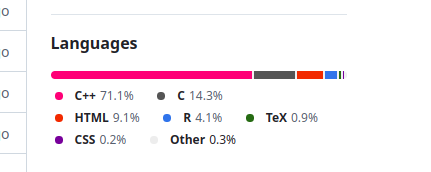
\includegraphics[keepaspectratio]{images/stringi-code.png}}

}

\caption{\texttt{stringi} package sourcecode.}

\end{figure}%

In Julia, you won't need other language to get speed close to C. That's
way they say that Julia
\href{https://juliadatascience.io/julia_accomplish\#sec:two_language}{solves
the two language problem}. Julia packages are almost always 100\% Julia,
which means that you can look to its sourcecode and learn a lot.

\begin{figure}[H]

{\centering \pandocbounded{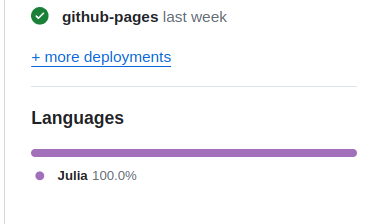
\includegraphics[keepaspectratio]{images/flux.png}}

}

\caption{Images that make you cry: the deep learning package
\href{https://github.com/FluxML/Flux.jl}{Flux.jl}.}

\end{figure}%

This is specially interesting if you read Julia Base sourcecode! How
does Julia define the maximum of a vector? Type

\begin{Shaded}
\begin{Highlighting}[]
\PreprocessorTok{@edit} \FunctionTok{maximum}\NormalTok{([}\FloatTok{1}\OperatorTok{:}\FloatTok{5}\NormalTok{;])}
\end{Highlighting}
\end{Shaded}

and you will see this:

\begin{figure}[H]

{\centering \pandocbounded{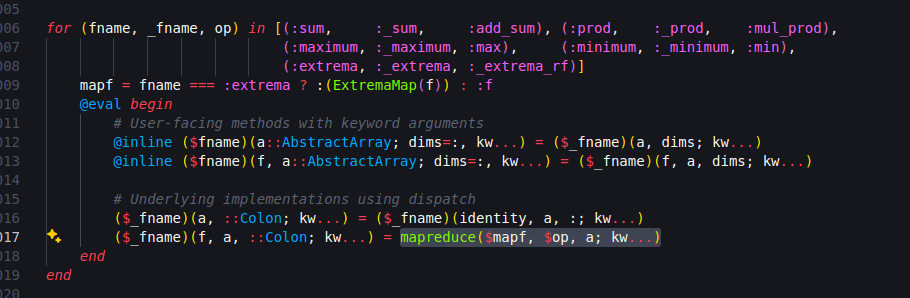
\includegraphics[keepaspectratio]{images/maximum-sourcecode.png}}

}

\caption{The sourcecode of the function maximum applied to a vector.}

\end{figure}%

It takes some time to grasp the meaning, but in the end it says ``apply
a mapreduce into the vector, using the max function on each pair of
numbers''. In R, the sourcecode is a sad \texttt{.Primitive("max")}.

In Julia, to obtain maximum performance, you need to follow just two
principles, as quoted from the excellent
\href{https://modernjuliaworkflows.org/optimizing/}{Modern Julia
Workflows}:

\begin{itemize}
\tightlist
\item
  Ensure that the compiler can infer the type of every variable.
\item
  Avoid unnecessary (heap) allocations.
\end{itemize}

For me, it sounds easier than learn C++.

\subsection{No need to vectorize code; loops, maps and broadcast are
fast
enough}\label{no-need-to-vectorize-code-loops-maps-and-broadcast-are-fast-enough}

Tired of writing loops? Julia has a special notation \texttt{.} (yes, a
dot) to apply \emph{any} function to a vector/array/iterable-object;
this is called
\href{https://docs.julialang.org/en/v1/manual/arrays/\#Broadcasting}{\emph{broadcasting}}.
For example, you can apply the \texttt{power2} function in a vector as
easy as

\begin{Shaded}
\begin{Highlighting}[]
\CommentTok{\#julia}
\CommentTok{\# define power2 for numbers}
\FunctionTok{power2}\NormalTok{(x) }\OperatorTok{=}\NormalTok{ x}\OperatorTok{\^{}}\FloatTok{2}\NormalTok{;}

\CommentTok{\# apply in vectors}
\FunctionTok{power2}\NormalTok{.(}\FloatTok{1}\OperatorTok{:}\FloatTok{10}\NormalTok{)}
\end{Highlighting}
\end{Shaded}

\begin{verbatim}
10-element Vector{Int64}:
   1
   4
   9
  16
  25
  36
  49
  64
  81
 100
\end{verbatim}

or in a matrix

\begin{Shaded}
\begin{Highlighting}[]
\CommentTok{\#julia}
\NormalTok{X }\OperatorTok{=} \FunctionTok{reshape}\NormalTok{([}\FloatTok{1}\OperatorTok{:}\FloatTok{16}\NormalTok{;], (}\FloatTok{4}\NormalTok{, }\FloatTok{4}\NormalTok{))}
\end{Highlighting}
\end{Shaded}

\begin{verbatim}
4×4 Matrix{Int64}:
 1  5   9  13
 2  6  10  14
 3  7  11  15
 4  8  12  16
\end{verbatim}

\begin{Shaded}
\begin{Highlighting}[]
\CommentTok{\#julia}
\FunctionTok{power2}\NormalTok{.(X)}
\end{Highlighting}
\end{Shaded}

\begin{verbatim}
4×4 Matrix{Int64}:
  1  25   81  169
  4  36  100  196
  9  49  121  225
 16  64  144  256
\end{verbatim}

When using infix functions like \texttt{+} or \texttt{=}, you put the
dot before the operator, as in

\begin{Shaded}
\begin{Highlighting}[]
\CommentTok{\#julia}
\NormalTok{[}\FloatTok{1}\OperatorTok{:}\FloatTok{5}\NormalTok{;] }\OperatorTok{.+} \FloatTok{10}
\end{Highlighting}
\end{Shaded}

\begin{verbatim}
5-element Vector{Int64}:
 11
 12
 13
 14
 15
\end{verbatim}

In R, you always try to avoid loops because they are \emph{slow}.
Suppose you have a vector and want to sum 1 to every entry. As an
experienced R programmer, you look for a vectorized approach:

\begin{Shaded}
\begin{Highlighting}[]
\CommentTok{\# R}
\NormalTok{f1\_vec }\OtherTok{=} \ControlFlowTok{function}\NormalTok{(x) \{}
\NormalTok{    y }\OtherTok{=}\NormalTok{ x }\SpecialCharTok{+} \DecValTok{1}
\NormalTok{\}}
\end{Highlighting}
\end{Shaded}

instead of a loop

\begin{Shaded}
\begin{Highlighting}[]
\CommentTok{\# R}
\NormalTok{f1\_loop }\OtherTok{=} \ControlFlowTok{function}\NormalTok{(x) \{}
\NormalTok{    y }\OtherTok{=}\NormalTok{ x}
    \ControlFlowTok{for}\NormalTok{ (i }\ControlFlowTok{in} \FunctionTok{seq\_along}\NormalTok{(x)) y[i] }\OtherTok{=}\NormalTok{ x[i] }\SpecialCharTok{+} \DecValTok{1}
\NormalTok{    y}
\NormalTok{\}}
\end{Highlighting}
\end{Shaded}

or a even a \texttt{purrr::map} approach (if you are in a functional
programming mood)

\begin{Shaded}
\begin{Highlighting}[]
\CommentTok{\#R}
\NormalTok{f1\_map }\OtherTok{=} \ControlFlowTok{function}\NormalTok{(x) \{}
\NormalTok{    purrr}\SpecialCharTok{::}\FunctionTok{map\_dbl}\NormalTok{(x, \textbackslash{}(xi) xi }\SpecialCharTok{+} \DecValTok{1}\NormalTok{)}
\NormalTok{\}}
\end{Highlighting}
\end{Shaded}

because the first options is faster. We can see the difference:

\begin{Shaded}
\begin{Highlighting}[]
\CommentTok{\# R}
\NormalTok{x }\OtherTok{=} \DecValTok{1}\SpecialCharTok{:}\DecValTok{100000}

\NormalTok{bench}\SpecialCharTok{::}\FunctionTok{mark}\NormalTok{(}
    \FunctionTok{f1\_vec}\NormalTok{(x)}
\NormalTok{    ,}\FunctionTok{f1\_loop}\NormalTok{(x)}
\NormalTok{    ,}\FunctionTok{f1\_map}\NormalTok{(x)}
\NormalTok{    ,}\AttributeTok{relative =} \ConstantTok{TRUE}
\NormalTok{)}
\end{Highlighting}
\end{Shaded}

\begin{verbatim}
RObject{VecSxp}
# A tibble: 3 × 13
  expression   min median `itr/sec` mem_alloc `gc/sec` n_itr  n_gc total_time
  <bch:expr> <dbl>  <dbl>     <dbl>     <dbl>    <dbl> <int> <dbl>   <bch:tm>
1 f1_vec(x)    1      1       125.       1        11.1   797    11      500ms
2 f1_loop(x)  44.2   14.6      10.4      1.03      1      67     1      506ms
3 f1_map(x)  542.   151.        1        1.00     32.2     7    35      550ms
# ℹ 4 more variables: result <list>, memory <list>, time <list>, gc <list>
\end{verbatim}

In my machine, the loop is \textasciitilde12x slower and the map
\textasciitilde145x slower than the vectorized version.

The biggest problem for an R user is when the function you want to apply
have no vectorized form. I usually have to make some kludges\footnote{or
  \href{https://pt.wikipedia.org/wiki/Gambiarra}{gambiarras}, in
  Brasileirês} with dplyr verbs to do something that is much more
logical when written with a loop/map.

In Julia, the three approachs are similar:

\begin{Shaded}
\begin{Highlighting}[]
\CommentTok{\#julia}
\FunctionTok{f1\_vec}\NormalTok{(x) }\OperatorTok{=}\NormalTok{ x }\OperatorTok{.+} \FloatTok{1}\NormalTok{;}

\KeywordTok{function} \FunctionTok{f1\_loop}\NormalTok{(x)}
\NormalTok{    y }\OperatorTok{=} \FunctionTok{similar}\NormalTok{(x)}
    \PreprocessorTok{@inbounds} \ControlFlowTok{for}\NormalTok{ i }\OperatorTok{∈} \FunctionTok{eachindex}\NormalTok{(x) y[i] }\OperatorTok{=}\NormalTok{ x[i] }\OperatorTok{+} \FloatTok{1} \ControlFlowTok{end}
\NormalTok{    y}
\KeywordTok{end}\NormalTok{;}

\KeywordTok{function} \FunctionTok{f1\_map}\NormalTok{(x)}
    \FunctionTok{map}\NormalTok{(x) }\ControlFlowTok{do}\NormalTok{ xi}
\NormalTok{        xi }\OperatorTok{+} \FloatTok{1} 
    \ControlFlowTok{end}
\KeywordTok{end}\NormalTok{;}
\end{Highlighting}
\end{Shaded}

\begin{Shaded}
\begin{Highlighting}[]
\CommentTok{\#julia}
\ImportTok{using} \BuiltInTok{BenchmarkTools;}
\NormalTok{x }\OperatorTok{=}\NormalTok{ [}\FloatTok{1}\OperatorTok{:}\FloatTok{100000}\NormalTok{;];}

\PreprocessorTok{@benchmark} \FunctionTok{f1\_vec}\NormalTok{(}\OperatorTok{$}\NormalTok{x)}
\end{Highlighting}
\end{Shaded}

\begin{verbatim}
BenchmarkTools.Trial: 10000 samples with 1 evaluation per sample.
 Range (min … max):  57.650 μs …  4.640 ms  ┊ GC (min … max): 0.00% … 97.43%
 Time  (median):     74.799 μs              ┊ GC (median):    0.00%
 Time  (mean ± σ):   89.406 μs ± 79.381 μs  ┊ GC (mean ± σ):  6.13% ±  9.49%

   █ ▆                                                         
  ▅█▅█▆▃▃▃▃▃▃▃▃▃▃▃▃▃▂▂▂▂▂▂▂▂▂▂▂▂▂▂▂▂▂▂▂▁▂▁▁▁▁▁▂▁▂▂▂▂▂▂▂▂▂▂▂▂▂ ▃
  57.6 μs         Histogram: frequency by time         340 μs <

 Memory estimate: 781.30 KiB, allocs estimate: 2.
\end{verbatim}

\begin{Shaded}
\begin{Highlighting}[]
\CommentTok{\#julia}
\PreprocessorTok{@benchmark} \FunctionTok{f1\_loop}\NormalTok{(}\OperatorTok{$}\NormalTok{x)}
\end{Highlighting}
\end{Shaded}

\begin{verbatim}
BenchmarkTools.Trial: 10000 samples with 1 evaluation per sample.
 Range (min … max):  54.755 μs … 989.312 μs  ┊ GC (min … max): 0.00% … 44.21%
 Time  (median):     75.891 μs               ┊ GC (median):    0.00%
 Time  (mean ± σ):   91.340 μs ±  51.966 μs  ┊ GC (mean ± σ):  5.52% ±  9.46%

   █▅▁▃                                                         
  ▃████▅▅▅▄▄▄▄▄▃▃▃▃▃▃▃▂▂▂▂▂▂▂▂▂▂▂▂▂▂▁▂▂▂▂▂▂▂▂▂▂▂▂▂▂▂▂▂▂▂▂▂▂▂▂▂ ▃
  54.8 μs         Histogram: frequency by time          358 μs <

 Memory estimate: 781.30 KiB, allocs estimate: 2.
\end{verbatim}

\begin{Shaded}
\begin{Highlighting}[]
\CommentTok{\#julia}
\PreprocessorTok{@benchmark} \FunctionTok{f1\_map}\NormalTok{(}\OperatorTok{$}\NormalTok{x)}
\end{Highlighting}
\end{Shaded}

\begin{verbatim}
BenchmarkTools.Trial: 10000 samples with 1 evaluation per sample.
 Range (min … max):  55.787 μs … 677.214 μs  ┊ GC (min … max): 0.00% … 60.28%
 Time  (median):     76.544 μs               ┊ GC (median):    0.00%
 Time  (mean ± σ):   93.394 μs ±  51.262 μs  ┊ GC (mean ± σ):  5.32% ±  9.40%

   █▄▅▅                                                         
  ▂████▄▄▄▄▄▄▄▄▄▃▃▃▃▃▃▂▂▂▂▂▂▂▂▂▂▂▂▂▂▂▂▂▂▂▂▂▂▂▂▂▂▂▁▂▂▁▁▂▂▂▂▂▂▂▂ ▃
  55.8 μs         Histogram: frequency by time          360 μs <

 Memory estimate: 781.30 KiB, allocs estimate: 2.
\end{verbatim}

This means that in Julia it is usual to \emph{define a function using a
scalar type} (a Number like Float64/Int or a String) \emph{and then use
broadcast} to apply the function to vectors/matrices/etc. No need to
create vectorized forms of functions anymore!

\subsection{The compiler is your
friend}\label{the-compiler-is-your-friend}

Sometimes you write code that won't make your parents proud. Suppose you
create a function that sums all the numbers from 1 to a given
\texttt{n}:

\begin{Shaded}
\begin{Highlighting}[]
\KeywordTok{function} \FunctionTok{f\_sum}\NormalTok{(n)}
\NormalTok{    s }\OperatorTok{=} \FloatTok{0}
    \ControlFlowTok{for}\NormalTok{ i }\KeywordTok{in} \FloatTok{1}\OperatorTok{:}\NormalTok{n}
\NormalTok{        s }\OperatorTok{+=}\NormalTok{ i}
    \ControlFlowTok{end}

\NormalTok{    s}
\KeywordTok{end}\NormalTok{;}
\end{Highlighting}
\end{Shaded}

In R, the language will obediently execute each iteration of the loop,
as you demanded, and it will take forever. You are the boss.

But in Julia, we have this curious phenomena:

\begin{Shaded}
\begin{Highlighting}[]
\PreprocessorTok{@time} \FunctionTok{f\_sum}\NormalTok{(}\FloatTok{100}\NormalTok{)}
\end{Highlighting}
\end{Shaded}

\begin{verbatim}
  0.000001 seconds
\end{verbatim}

\begin{verbatim}
5050
\end{verbatim}

\begin{Shaded}
\begin{Highlighting}[]
\PreprocessorTok{@time} \FunctionTok{f\_sum}\NormalTok{(}\FloatTok{100\_000}\NormalTok{)}
\end{Highlighting}
\end{Shaded}

\begin{verbatim}
  0.000001 seconds
\end{verbatim}

\begin{verbatim}
5000050000
\end{verbatim}

\begin{Shaded}
\begin{Highlighting}[]
\PreprocessorTok{@time} \FunctionTok{f\_sum}\NormalTok{(}\FloatTok{100\_000\_000}\NormalTok{)}
\end{Highlighting}
\end{Shaded}

\begin{verbatim}
  0.000001 seconds
\end{verbatim}

\begin{verbatim}
5000000050000000
\end{verbatim}

How is it possible that it took the same time to run 100 iterations and
100 million iterations? The magic is the compiler: it understood that
what you are doing is the sum of the terms of an
\href{https://en.wikipedia.org/wiki/Arithmetic_progression}{arithmetic
progression}. The legend says that Gauss deduced the formula for its
sum, and the compiler did the same for you. No need to be as smart as
Gauss while using Julia.

Julia is a
\href{https://docs.julialang.org/en/v1/\#man-julia-compared-other-languages}{just-in-time
(JIT) compiled language}, which means that each function is compiled
when you first execute it. The ``time to first compile'' was a problem
in the past, but from Julia 1.8 onwards it is not a big deal. The
compiler is your friend, and almost always you can trust him.

\subsection{Multiple dispatch and type
system}\label{multiple-dispatch-and-type-system}

A type system is a way to organize data types within an hierarchy. Think
of it as mathematical sets: you have the real numbers, and inside it are
the rationals, the integers, the naturals, etc. Each one of these types
store data into memory in a different manner (integers can be stored
more efficiently than arbitrary real numbers, for example). Julia has a
really nice \href{https://docs.julialang.org/en/v1/manual/types/}{type
system}. Let's see some examples to better understand it.

Consider the \texttt{print} function in R. It is a \emph{generic}
function, which means that its behaviour depends on the class/type of
its first argument. This can be seen when we look to its misterious
source code:

\begin{figure}[H]

{\centering \pandocbounded{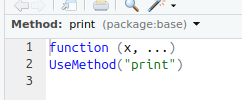
\includegraphics[keepaspectratio]{images/print-code.png}}

}

\caption{The \texttt{print} function sourcecode.}

\end{figure}%

which means that \texttt{print} will use several \texttt{methods}
(implementations/pieces-of-code), one for each class/type. Actually, R
just creates a different function for each class, with the pattern
\texttt{\{function\}.\{class\}}:

\begin{figure}[H]

{\centering \pandocbounded{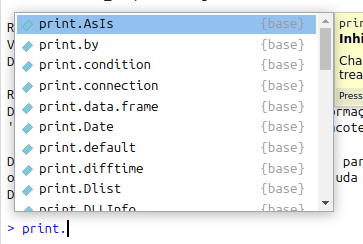
\includegraphics[keepaspectratio]{images/print-methods.png}}

}

\caption{Each method/implementation of the generic function
\texttt{print}.}

\end{figure}%

In Julia, \emph{every function is generic}. We can use the same function
name and define different behaviours/implementations for each
combination of classes/types of its arguments. We saw above the
implementation of the \texttt{maximum} function in Julia for an
arbitrary vector of numbers. But what if the vector is of a different
kind, for which it is easier to determine its maximum?

Take, for example, the object

\begin{Shaded}
\begin{Highlighting}[]
\NormalTok{x }\OperatorTok{=} \FloatTok{1}\OperatorTok{:}\FloatTok{10}
\end{Highlighting}
\end{Shaded}

\begin{verbatim}
1:10
\end{verbatim}

It is \emph{not} a vector (to create a usual vector from 1 to 10, you
type \texttt{{[}1:10;{]}}). Actually, its type is

\begin{Shaded}
\begin{Highlighting}[]
\FunctionTok{typeof}\NormalTok{(x)}
\end{Highlighting}
\end{Shaded}

\begin{verbatim}
UnitRange{Int64}
\end{verbatim}

and its type hierarchy is

\begin{Shaded}
\begin{Highlighting}[]
\BuiltInTok{Base}\NormalTok{.}\FunctionTok{show\_supertypes}\NormalTok{(}\FunctionTok{typeof}\NormalTok{(x))}
\end{Highlighting}
\end{Shaded}

\begin{verbatim}
UnitRange{Int64} <: AbstractUnitRange{Int64} <: OrdinalRange{Int64, Int64} <: AbstractRange{Int64} <: AbstractVector{Int64} <: Any
\end{verbatim}

So \texttt{x} is a much simpler object than a vector: it is an
increasing sequence of integer numbers, each 1 unity bigger than the
previous one. It makes sense then that the \texttt{maximum} function can
be defined much more simpler for an object of type
\texttt{UnitRange\{Int64\}}: the biggest element is always the last.

If you look at the sourcecode

\begin{Shaded}
\begin{Highlighting}[]
\PreprocessorTok{@edit} \FunctionTok{maximum}\NormalTok{(}\FloatTok{1}\OperatorTok{:}\FloatTok{10}\NormalTok{)}
\end{Highlighting}
\end{Shaded}

you will get

\begin{Shaded}
\begin{Highlighting}[]
\FunctionTok{maximum}\NormalTok{(r}\OperatorTok{::}\DataTypeTok{AbstractUnitRange}\NormalTok{) }\OperatorTok{=} \FunctionTok{isempty}\NormalTok{(r) ? }\FunctionTok{throw}\NormalTok{(}\FunctionTok{ArgumentError}\NormalTok{(}\StringTok{"range must be non{-}empty"}\NormalTok{)) }\OperatorTok{:} \FunctionTok{last}\NormalTok{(r)}
\end{Highlighting}
\end{Shaded}

which is exactly what we thought:

\begin{quote}
is the range non-empty? Then take de last element; otherwise, an error.
\end{quote}

The function \texttt{last} is defined for every children of type
\texttt{AbstractUnitRange}, and so \texttt{maximum} is well defined.

In summary: Julia has an arbitrary \texttt{maximum} function for
arbitrary vectors, but has specialized methods for some other specific
types. This is a common pattern in Julia, and much of its performance
depends on this.

\subsection{Macros rewrite code without
typing}\label{macros-rewrite-code-without-typing}

\href{https://docs.julialang.org/en/v1/manual/metaprogramming/}{Macros}
are one of the most powerful tools in Julia. They rewrite your code
before executing it: it is a metaprogramming technique. When creating
macros, you will have to understand how a bunch of characters are
interpreted by the language and executed as code. This means that macros
can rewrite pieces of code and add functionalities that are not possible
simply with functions.

We already used some macros on this notebook; they all start with the
\texttt{@} symbol.

How much time does it take to calculate the sin of a million numbers?

\begin{Shaded}
\begin{Highlighting}[]
\PreprocessorTok{@time} \FunctionTok{sin}\NormalTok{.(}\FloatTok{1}\OperatorTok{:}\FloatTok{1\_000\_000}\NormalTok{);}
\end{Highlighting}
\end{Shaded}

\begin{verbatim}
  0.031893 seconds (2 allocations: 7.629 MiB, 41.00% gc time)
\end{verbatim}

Do you have a loop and want to see a progress bar? No need to change the
code inside the loop:

\begin{Shaded}
\begin{Highlighting}[]
\ImportTok{using} \BuiltInTok{ProgressMeter;}

\PreprocessorTok{@showprogress} \ControlFlowTok{for}\NormalTok{ i }\KeywordTok{in} \FloatTok{1}\OperatorTok{:}\FloatTok{10}
    \FunctionTok{sleep}\NormalTok{(}\FloatTok{0.1}\NormalTok{)}
\ControlFlowTok{end}
\end{Highlighting}
\end{Shaded}

\begin{verbatim}
Progress:  20%|████████▎                                |  ETA: 0:00:08Progress: 100%|█████████████████████████████████████████| Time: 0:00:03
\end{verbatim}

As we've seen, even the tidyverse could be recreated in Julia using
macros!

\subsection{Multithreading is trivial}\label{multithreading-is-trivial}

\href{https://docs.julialang.org/en/v1/manual/multi-threading/}{Multithreading}
(or parallel computing) is when your code uses more than one processor
at the same time. Multithreading in R is a bit complicated and actually
create copies of the R process that comunicates with the main process.
There is a
\href{https://www.futureverse.org/packages-overview.html}{\texttt{futureverse}}
to deal with that in R, and plans like \texttt{callr} or
\texttt{multisession} to define how these extra R sessions will be
created and mantained.

In Julia, multithreading is as easy as appending a macro before a loop:

\begin{Shaded}
\begin{Highlighting}[]
\BuiltInTok{Threads}\NormalTok{.}\PreprocessorTok{@threads} \ControlFlowTok{for}\NormalTok{ i }\OperatorTok{=} \FloatTok{1}\OperatorTok{:}\FloatTok{10}
\NormalTok{    a[i] }\OperatorTok{=} \BuiltInTok{Threads}\NormalTok{.}\FunctionTok{threadid}\NormalTok{()}
\ControlFlowTok{end}
\end{Highlighting}
\end{Shaded}

If you want a multithread version of \texttt{map} and \texttt{reduce}
and so on, check \href{https://github.com/tkf/ThreadsX.jl}{ThreadsX.jl}.

Multithread is recommended when you: - have some spare RAM; - have more
than 1 processor; - want to apply some function on a list of things that
take some time idling (for example, waiting for an API return something)
or are not RAM-heavy (calculating small distance matrices).

My tipical use case is when I have a large dataframe and want to apply a
function to several parts of it, based on a grouping variable. I split
the dataframe into a vector of dataframes (with \texttt{groupby} and
\texttt{collect}) and then apply the function in parallel.

Another use is the following: suppose you want to create an API to serve
5 simultaneous users requesting data all day. In R you will use
\href{https://www.rplumber.io/}{\texttt{plumber}} and make lots of
\texttt{future\_promise} calls. In Julia, just use
\href{https://oxygenframework.github.io/Oxygen.jl/stable/\#Multithreading-and-Parallelism}{\texttt{Oxygen.jl}}
without any need to change your code: the requests are made in parallel.

\subsection{Packages are a joy to use}\label{packages-are-a-joy-to-use}

In R, you have 2 options to call a function from another package:

\begin{itemize}
\tightlist
\item
  use \texttt{library(PACKAGE)}, which imports \emph{every} function
  from PACKAGE to your namespace;
\item
  use \texttt{PACKAGE::FUNCTION} every time you want to use a function.
\end{itemize}

Packages like \href{https://klmr.me/box/}{\texttt{box}} are a more
``Pythonesque'' approach to importing libraries, and allow to import
just some parts of a package.

In Julia, a package is just a module, and you have:

\begin{itemize}
\tightlist
\item
  \texttt{using\ PACKAGE} is analogous to R \texttt{library(PACKAGE)};
\item
  \texttt{import\ PACKAGE} and then \texttt{PACKAGE.FUNCTION} in every
  call;
\item
  \texttt{using\ PACKAGE:\ FUNCTION1,\ FUNCTION2} will import only these
  2 functions from PACKAGE.
\end{itemize}

The best part, however, is the ability to create modules inside modules.
For example, if you have a mega package to do all your data analysis in
your work, you can have a module about Reports, another one with APIs
and so on. Importing then can be done with

\begin{Shaded}
\begin{Highlighting}[]
\ImportTok{using} \BuiltInTok{MyPackage.Reports}

\CommentTok{\# or}
\ImportTok{import} \BuiltInTok{MyPackage.APIs}\NormalTok{ as API}

\NormalTok{MD.}\FunctionTok{api1}\NormalTok{()}
\end{Highlighting}
\end{Shaded}

This approach resembles a little the idea of namespaces in
\href{https://mastering-shiny.org/scaling-modules.html}{shiny modules},
and using \texttt{box} is how the
\href{https://appsilon.github.io/rhino/articles/explanation/box-modules.html}{\texttt{rhino}}
emulate the ``module inside module'' thing.

\subsection{Math symbols for the math
enthusiasts}\label{math-symbols-for-the-math-enthusiasts}

Examples of correct Julia code:

\begin{Shaded}
\begin{Highlighting}[]
\NormalTok{[}\FloatTok{1}\NormalTok{, }\FloatTok{2}\NormalTok{] }\OperatorTok{∩}\NormalTok{ [}\FloatTok{2}\NormalTok{, }\FloatTok{3}\NormalTok{]}
\end{Highlighting}
\end{Shaded}

\begin{verbatim}
1-element Vector{Int64}:
 2
\end{verbatim}

\begin{Shaded}
\begin{Highlighting}[]
\FloatTok{2} \OperatorTok{∈}\NormalTok{ [}\FloatTok{2}\NormalTok{, }\FloatTok{3}\NormalTok{]}
\end{Highlighting}
\end{Shaded}

\begin{verbatim}
true
\end{verbatim}

\begin{Shaded}
\begin{Highlighting}[]
\FunctionTok{f}\NormalTok{(r) }\OperatorTok{=} \ConstantTok{π}\OperatorTok{*}\NormalTok{r}\OperatorTok{\^{}}\FloatTok{2}

\FunctionTok{f}\NormalTok{(}\FloatTok{3}\NormalTok{)}
\end{Highlighting}
\end{Shaded}

\begin{verbatim}
28.274333882308138
\end{verbatim}

\begin{Shaded}
\begin{Highlighting}[]
\CommentTok{\# Euler\textquotesingle{}s identity}
\ConstantTok{ℯ}\OperatorTok{\^{}}\NormalTok{(}\ConstantTok{im} \OperatorTok{*} \ConstantTok{π}\NormalTok{) }\OperatorTok{+} \FloatTok{1} \OperatorTok{|\textgreater{}}\NormalTok{ round}
\end{Highlighting}
\end{Shaded}

\begin{verbatim}
0.0 + 0.0im
\end{verbatim}

\begin{center}\rule{0.5\linewidth}{0.5pt}\end{center}

If I convinced you or sparked just a little interest, you can start your
own journey in Julialand with the suggested steps:

\begin{enumerate}
\def\labelenumi{\arabic{enumi}.}
\tightlist
\item
  \href{https://modernjuliaworkflows.org}{Modern Julia Workflows}:
  install Julia, setup your IDE and learn the basics of how to run code.
\item
  \href{https://docs.julialang.org/en/v1/manual/getting-started/}{The
  Julia docs} are excellent: need to understand more about
  \href{https://docs.julialang.org/en/v1/manual/variables/}{variables}?
  What about the
  \href{https://docs.julialang.org/en/v1/manual/functions/}{scope of
  functions}?
  \href{https://docs.julialang.org/en/v1/manual/types/}{Types} is
  certainly worth a read!
\item
  \href{https://benlauwens.github.io/ThinkJulia.jl/latest/book.html}{Think
  Julia}, by Be Lauwens and Allen Doeney: similar to Think Python, but
  better!
\item
  Questions? Go to the \href{https://discourse.julialang.org/}{Julia
  Discourse}.
\item
  For a list of really nice packages, see
  \href{https://gensjulia.pages.dev/data-science/\#general-purpose}{this
  repo}.
\end{enumerate}

Have a good trip!




\end{document}
